\documentclass[12pt]{report}
% Pacchetti necessari
\usepackage{multirow}
\usepackage{amsmath}
\usepackage{amssymb}
\usepackage{graphicx}
\usepackage{booktabs}
\usepackage{epstopdf}
\usepackage[utf8]{inputenc}
\usepackage{listings}
\usepackage{geometry}
\usepackage{physics}
\usepackage{tabularx}
\usepackage{matlab-prettifier}
\usepackage{subcaption}
\usepackage{algpseudocode}
\usepackage{etoolbox}
\usepackage{mathtools}
\usepackage{nccmath}
\usepackage{algorithm}
\geometry{left=2.5cm, right=2.5cm, top=2.5cm, bottom=3.5cm}
\usepackage{graphicx} % Required for inserting images
\usepackage{mathtools}
\usepackage{amsmath}
\DeclarePairedDelimiter\ceil{\lceil}{\rceil}
\DeclarePairedDelimiter\floor{\lfloor}{\rfloor}
% Pacchetti per intestazioni e piè di pagina
\usepackage{fancyhdr}
\usepackage{lastpage}
\usepackage[backend=biber,style=numeric]{biblatex}
\addbibresource{biblio.bib}  % Point to your .bib file

\begin{document}
\pagestyle{fancy}

% Impostazione dell'altezza dell'intestazione
\setlength{\headheight}{1cm} % Altezza dell'intestazione; regola questo valore secondo necessità


% Impostazione della intestazione
\fancyhead[L] {} % Modifica il percorso e la dimensione del logo
\fancyhead[C]{}
\fancyhead[R]{\leftmark{}}


% Impostazione del piè di pagina
\fancyfoot[L]{}
\fancyfoot[C]{\thepage} % Numero di pagina centrato nel piè di pagina
\fancyfoot[R]{}

% Definisci la spaziatura verticale per centrare il testo nell'intestazione
\fancyhead[R]{\vspace{10pt} \rightmark{}} % R = Destra, spostato di 10pt verso il basso

\begin{titlepage}
    \centering
    
    % Logo dell'università
    
\includegraphics[width=0.6\textwidth]{logounipa.png} 
    
    \vspace{1cm}
    
    % Nome dell'università
    {\large Università degli Studi di Palermo \par}
    
    \vspace{1cm}
    
    % Nome della materia
    {\Large \bfseries Analisi Intelligente dei Segnali \par}
    
    \vspace{1.5cm}
    
    % Nome del progetto con grassetto più marcato
    {\Huge \textbf{Speech Features per i tasks di \\ Speaker Identification e Verification} \par}
    \vspace{2cm}
    
    % Nome del docente a sinistra e nome dello studente a destra
    % Nome del docente a sinistra e nome dello studente a destra
    \noindent
    \begin{minipage}{0.45\textwidth}
        \raggedright
        {\large \bfseries Docente:} \\
        {\large Sabato Marco Siniscalchi}
    \end{minipage}
    \hfill
    \begin{minipage}{0.45\textwidth}
        \raggedleft
        {\large \bfseries Autore:} \\
        {\large Costa Gabriele Nicolò}
    \end{minipage}


    
    \vspace{2cm}
    
    % Nome del corso
    {\Large \bfseries Corso di Laurea \par}
    {\large Ingegneria Informatica LM-32 \par}

    \vspace{2cm}

    % Anno accademico centrato
    {\Large \bfseries Anno Accademico 2024/25 \par}
    
\end{titlepage}

\tableofcontents
\chapter{Introduzione}
Nel contesto dell'analisi intelligente dei segnali un task molto importante e di notevole interesse scientifico-industriale 
è il riconoscimento del parlante o in genere dell'identificazione di chi parla a discapito di impostori. Il seguente progetto affronta la tematica
della \textbf{speaker identification} e della \textbf{speaker verification}, analizzando le principali tecniche che permettono di ottenere
una rappresentazione alternativa a partire dalle tracce audio al fine di realizzare il riconoscimento degli speakers. 
Verranno quindi appprofondite le tecniche utilizzate e le \textbf{features} che entrerannno in gioco, analizzando come e quali sistemi permettono l'analisi di queste
caratteristiche. Infine verrà condotta una fase sperimentale dove verranno confrontate diverse tecniche e metodologie proposte in ambito di ricerca. \\
Il seguente progetto è strutturato nel seguente modo:
\begin{itemize}
    \item Il capitolo \ref{ch:speakerID} prenderà in considerazione il problema, analizzando cosa viene fatto in letteratura scientifica
    \item Il capitolo \ref{ch:features} analizzerà quali sono le features largamente utilizzate per poter effettuare speaker identification e verification 
    \item Il capitolo \ref{ch:speakermodels} fornirà una overview dei sistemi utilizzati per analizzare le features descritte prima, entrando anche nel dettaglio dell'architettura utilizzata
        per realizzare speaker identification e verification in un unica pipeline integrata
    \item Il capitolo \ref{ch:esperimenti} infine valuterà gli esperimenti condotti, descrivendo dataset e risultati ottenuti
\end{itemize}

% Nella introduzione parlare delle idee del progetto in generale e in quale aspetto ci siamo
% concentrati e perché, parlando anche di possibili scenari applicativi e motivazioni.
% Descrivere nella pratica (prendendo spunto dai vari paper scientifici) 
% di cosa tratteremo:
% \begin{itemize}
%     \item Capitolo 1: speaker identification e Verification, pipeline e come fare il tutto
%     \item Capitolo 2: speech featues, con particolare appiglio su MFCC, Mel Filterbanks, I-Vector, X-Vector
%     \item Capitolo 3: Speaker Model e Backend, introduzione alle tecniche utilizzate finora, dicendo quelle che analizzeremo
%     \item Capitolo 4: Sezione sperimentale 
%     \item Capitolo 4.1: descrizione del dataset utilizzato e della pipeline di lavoro, analizzando quali speaker stiamo utilizzando (in termini di Spettrogrammi e Classificazione maschio femmina)
%     \item Capitolo 4.1: utilizzo degli MFCC e descrizione dei risultati sperimentali sia per la identification che la verification con EER
%     \item Capitolo 4.2: utilizzo degli I-Vector e architettura della letteratura
%     \item Capitolo 4.3: utilizzo degli x-vector e arcitettura della letteratura per gli embeddings 
% \end{itemize}

\newpage
\chapter{Speaker Identification e Verification}
\label{ch:speakerID}

\section{Descrizione del problema}
Nel contesto dell'analisi intelligente dei segnali sappiamo che lavorando con sorgenti audio spesso ricorriamo ad una rappresentazione alternativa per ogni specifico 
segnale audio, chiamata appunto come rappresentazione di \textbf{features}, che possiamo usare per task diversi. \\
Uno dei task che da sempre è studio di lavori (sia per la sua applicabilità pratica nel settore industriale, che da un punto di vista di ricerca) è quello 
dello \text{Speaker Identification}. Infatti questo task trova grande interesse nei sistemi di riconoscimento biometrici, diventando quindi un punto cruciale nel 
settore della sicurezza informatica. In generale, i sistemi biometrici si basano sulle caratteristiche \textit{individuali e altamente discriminative} delle persone, 
presentando già il principale compito dei sistemi di riconoscimento: identificare correttamente le persone e riconoscere se ci sono degli utenti non autorizzati (o impostori), 
sulla base delle caratteristiche (o \textit{features}) di ogni singolo speaker. \\
Nel task della \textit{speaker identification}, il nostro obiettivo principale è cercare di estrarre dagli human speech di ogni singolo speaker una rappresentazione alternativa 
utile a rappresentare univocamente un soggetto, quindi costruire dei \textbf{Speaker Models}, che permettano poi di riconoscere i singoli utenti tramite una classificaione 
o pattern-matching in generale. Lo scopo dello \textit{speaker models} è quello  alla fine di creare un database di persone (quindi di profili) che conosco, al fine di avere 
abbastanza informazioni per poter riconoscere quel determinato speaker in seguito. 
Uno schema di funzionamento è riportato in \ref{fig:speakerschema} Il sistema viene diviso in due fasi:
\begin{itemize}
    \item una fase di training, o anche definita come \textit{enrolment}, dove acquisiamo audio da cui estrarre features da cui estrarre un database di speaker models
    \item Una fase di \textit{testing}, dove andiamo a valutare quanti speaker riusciamo correttamente a riconoscere 
\end{itemize}
Quando però realizziamo la fase di testing dobbiamo distinguere tra una identificazione definita \textit{closed-set}, ovvero abbiamo un insieme di identità che conosciamo (quindi abbiamo profilato) 
e dobbiamo distinguere gli uni dagli altri, ed una identificazione definita \textit{open-set}, dove invece dobbiamo identificare tra identità che conosciamo e quelle che invece non conosciamo 
e classifichiamo come sconosciute, o appunto impostori. \\
In questo contesto si inserisce la \textit{speaker verification}. Partiamo da una base di identification (dove quindi abbiamo un database di identità conosciute), e cerchiamo
di capire se un un nuovo speaker fa parte del nostro insieme o no. In questo caso il focus non è tanto l'identificazione, ma tanto il rejection dell'utente nel caso in cui 
non faccia realmente parte del mio insieme di identità conosciute. Facendo un esempio banale, se un utente parla ad un sistema di riconoscimento e dice di essere un determinato utente (claimed ID), 
il sistema deve essere in grado di identificarlo correttamente (anche qui, closed-set o open-set) e di assegnargli una identità, eventualmente "bloccandolo" se troviamo che non è che dice di essere o non fa parte dell'insieme.
Parliamo quindi in questo caso di rejection e acceptance di un determinato speaker, per valutare correttamente il sistema, sulla base per esempio di uno score (compito di solito svolto dal Backend del sistema di verifica). \\

Inoltre, entrambi i task possono essere dipendenti o indipendenti dai vincoli lessicali \cite{tu2022survey}. Infatti distinguiamo tra \textit{Text-Indipendent} e \textit{Text-Dipendent},
sia in ottica Speaker Identification che Verification. Per vincolo lessicale intendiamo infatti che lo speaker deve dire una determinata sequenza di parole, che in pratica
corrisponde a pronunciare una \textit{keyword o passphrase}.

\begin{figure}[ht]
    \centering
    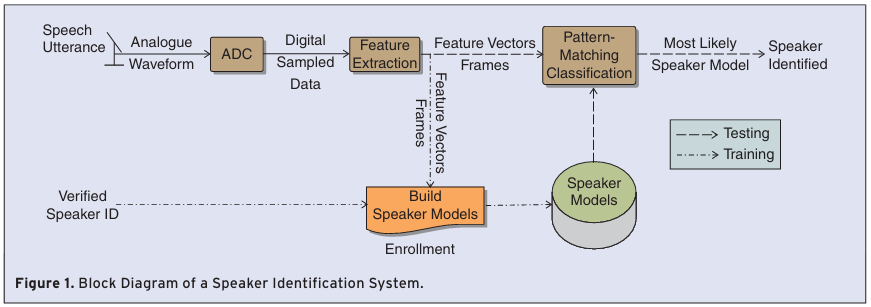
\includegraphics[width=1.0\textwidth]{./ch1/speaker_id.png}
    \caption{Sistema di Speaker identification, \protect\cite{togneri2011overview}}
    \label{fig:speakerschema}
\end{figure}


\begin{figure}[ht]
    \centering
    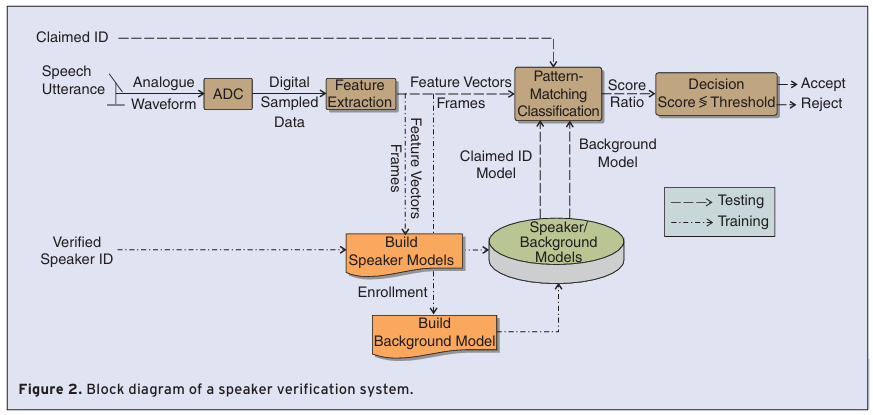
\includegraphics[width=1.0\textwidth]{./ch1/speaker_ver.png}
    \caption{Sistema di Speaker Verification, \protect\cite{togneri2011overview}}
    \label{fig:speakerschemaver}
\end{figure}

\section{Valutazione dei sistemi: metriche e metodologie}
Per poter correttamente valutare un sistema di identificazione e verifica delle identità dobbiamo basarci su specifiche metriche e metodologie.
Per quanto riguarda le metodologie, sia in open-set che closed-set, partiamo da un training set composto da segnali audio a cui applichiamo la classica analisi \textit{Short-Time},
al fine di poter effettuare operazioni di estrazione di features. Training e Testing sono composti da audio di speaker noti nel caso del task di Speaker Identification, da speaker diversi nel caso del task di Speaker Verification.

Per quanto riguarda le metriche da utilizzare, queste sono diverse a seconda del task. Nel task della identificazione è importante capire quanti utenti riusciamo a riconoscere
e distinguere correttamente, quindi valutare metriche come la \textit{precisione, la accuracy, la f1score} per ogni speaker e in maniera complessiva del sistema. 

Per quanto riguarda invece la verifica delle identità è più importante riconoscere quante persone riusciamo correttamente a riconoscere come intrusi e quindi bloccare e non far accedere al sistema. 
Quindi questo task è da vedere più come classificazione binaria che multiclasse, perché a noi interessano \textit{True Positive Rate (quante persone riusciamo correttamente a far passare)} e \textit{False Positive Rate (quante persone facciamo passare sebbene siano impostori)}.
Una metrica aggregata è la \textbf{Equal Error Rate (EER)}, metrica comune nei sistemi biometrici. Si riferisce al punto in cui il tasso di falsi accettamenti (\textbf{(FAR - False Acceptance Rate}) è uguale al tasso di falsi rifiuti (\textbf{FRR - False Rejection Rate}). 
In termini di TPR e TNR, la FAR è il complementare del TNR (percentuale di impostori correttamente identificati), quindi coincide con la FPR, mentre la TPR è il complementare della FRR (percentuale di parlanti autentici e correttamente accettati).
Un riassunto è riportato in Tab.\ref{tab:metriche}

\begin{table}[ht]
    \centering
    \renewcommand{\arraystretch}{1.4}
    \begin{tabular}{@{} m{4cm} m{5.5cm} m{6.5cm} @{}}
    \toprule
    \textbf{Task} & \textbf{Obiettivo} & \textbf{Metriche utilizzate} \\
    \midrule
    \textbf{Speaker Identification} (Closed-set) & 
    Riconoscere l'identità dello speaker tra un insieme noto di speakers (classificazione multiclasse). & 
    \begin{itemize}
    \item Accuracy
    \item Precision, Recall, F1-score (per classe e macro media)
    \end{itemize} \\
    \midrule
    \textbf{Speaker Verification} (Open-set) & 
    Verificare se uno speaker è chi dichiara di essere (classificazione binaria: accetta/rifiuta). & 
    \begin{itemize}
    \item True Positive Rate (TPR)
    \item False Positive Rate (FPR)
    \item False Acceptance Rate (FAR)
    \item False Rejection Rate (FRR)
    \item Equal Error Rate (EER)
    \end{itemize} \\

    \bottomrule
    \end{tabular}
    \caption{Task, obiettivi e metriche nei sistemi di speaker recognition}
    \label{tab:metriche}
\end{table}

\section{Scenari applicativi}
Come detto prima, questi task sono alla base sopratutto dei sistemi di riconoscimento biometrici, con particolare focus sia al riconoscimento che alla verifica dell'identità. 
Ques'ultimo aspetto diventa chiave e cruciale per i sistemi di sicurezza basati su riconoscimento della voce (\textit{biometrica dinamica}), per il controllo degli accessi o ulteriore fattore di autenticazione. \\
Lo scopo di questo progetto è quello di esplorare entrambi gli aspetti, con particolare focus alle tecniche principali che permettono di identificare gli speaker con metodologie basate sul Deep Learning, 
esplorando anche come un sistema di identificazione può essere traslato ed adattato in un sistema di verifica delle identità tramite classificazione binaria \textit{one-vs-others}, 
dove i nostri utenti VERI sono quelli del nostro dataset \textit{closed-set}, quelli invece FALSI (o impostori) sono quelli che non fanno parte del dataset.
\newpage
\chapter{Speech Features \& Embeddings}
\label{ch:features}
In molte applicazioni di speech processing è spesso conveniente ed utile avere una rappresentazione parametrica o alternativa dell'informazione
trasportata dal segnale. L'informazione trasportata dal segnale infatti include importanti fattori come il pitch period, il modello dell'impulso glottale,
l'eccitazione, il modello del tratto vocale: tutte informazioni utili a poter distinguere i diversi speaker in task come lo speaker identification
e lo speaker verification. L'obiettivo della Digital Speech Processing (DSP) è proprio quello di trovare metodi per poter elaborare i segnali speech audio
e poter quindi estrarre queste particolari informazioni in forma parametrica, avendo difatti una \textbf{rappresentazione alternativa} del segnale. 

Questo permette difatti di andare ad estrarre \textbf{speech features}, dunque parametri o caratteristiche, che possiamo dare in input a modelli di machine learning,
per permette alle reti di poter eseguire particolari combiti. Spesso però il machine learning ha una duplice valenza: è spesso usato sia come "modello" di elaborazione
delle features, sia come modello per estrarre rappresentazioni più raffinate delle features in input. Queste rappresentazioni più raffinate prendono il nome
di \textbf{speech embeddings}, e permettono di aggiungere un ulteriore informazione: permette difatti di aggregare i contributi di ogni singola features in ingresso,
cercando di ottenere rappresentazioni non lineari più complesse e talvolte più discriminanti.

\section{Speech Features}
In ogni caso, le proprietà dello speech cambiano lentamente nel tempo e nella frequenza. Per poter fronteggiare questo fenomeno si ricorre spesso a
metodi di analisi definiti come \textit{short time}, dove andiamo ad eseguire una analisi frame per frame. Questo deriva dal fatto che effettuando una analisi
short time a livello di frame, andiamo a processare singoli segmenti cui possiamo assumere abbiano proprietà fisse e permettono di estrarre le informazioni relative
per lo speech processing. Le metodologie di short time possono essere o basate su tempo o su frequenza. L'analisi time-domain è utile per andare ad isolare
segmenti dove è presente un pezzo di segnale \textit{voiced} oppure \textit{unvoiced}. Permette infatti di isoalre meglio segmenti dal rumore di fondo, utili per massimizzare
ulteriormente l'estrazione di features solo su segmenti definiti come voiced, ad esempio integrando un \textbf{Voice Activity Detector (VAD)}, che tronca andando a valutare
l'energia del segmento, ad esempio con analisi \textbf{Short Time Energy}. 

Tuttavia, nei task di \textbf{Speaker Verification} e \textbf{Speaker Identification}, conviene trattare di metodi short time basati sulla frequenza,
dal momento che molte informazioni riguardanti formanti e armoniche (utili per poter modellare un filtro che rappresenti il tratto vocale di una persona, quindi un modello
che riesce a parametrizzare), oltre che informazioni definibili come "percettive". Alcune features basate su metodi frequency-domain soon gli MFCCs (Mel Frequency Cepstral Coefficients).
Talvolta abbianiamo a queste features anche altri valori di derivata prima o seconda, per poter esprimere anche la variabilità dell'analisi short time, come i metodi Delta e Delta Delta.

\subsection{Cepstrum}
Il cepstrum è definito come la IDFT della log-magnitudo della DFT del segnale, ovvero:
\[ c[n] = F^{-1}[log(|F[x[n]]|) ]\]
Dove i due operatori sono la trasformata discreta di fourier DFT e la inverse DFT, la IDFT. A partire del cepstrum possiamo definire una rappresentazione alternativa,
ma non ci basta ancora: vorremmo smussare le attenuazioni, estraendo anche componenti come il pitch e sopratutto modellare l'inviluppo della trasformata stessa.
Tuttavia il cepstrum ci permette di poter separare la sorgente (voiced o treno di impulsi, e unvoiced o rumore gaussiano) ed il filtro (il tratto vocale), riuscendo quindi 
a modelleare in maniera compatta l'inviluppo spettrale. 

\subsection{Filter Banks e Mel-Scale}
Lo smooth con filterbanks riesce ad approssimare piccole variazioni, rendendo le features più robuste e meno rumorose. I filterbanks sono una serie di filtri
triangolari che permettono di andare a catturare selettivamente energia da uno specifico range di frequenze, pesando e sommando i bins spettrali in quella regione.
Questo processo permette di approssimare lo spettro e fornire una rappresentazione compatta di come l'energia è distribuita lungo le diverse bande di frequenza.
La rappresentazione smoothed cattura una forma complessiva dello spettro definita come "envelope", esaltando l'importanza delle features da un punto di vista percettivo.

\subsection{Mel-Frequency Cepstral Coefficients (MFCCs) }
La scala di Mel è una scala percettiva di pitch che approssima il modo in cui gli umani percepiscono i suoni delle frequenze. La scala di Mel è progettata per riflettere una relazione
non lineare tra la frequenza fisica e il tono percepito, risultando più sensibile alle basse frequenze, il quale riesce a farci a capire come l'orecchio umano percepisce
il suono. Formiamo quindi un filterbank cosicché i centri dei triangoli sono le frequenze che corrispondono a equal distanza sulla scala di mel. Effettuiamo quindi
una analisi short time dove applichiamo alla trasformata DFT i valori pesi del filtro filteranks:
\[ MF_m[r] = \frac{1}{A_r} \sum_{l=L_r}^{U_r} |V_r[k]X_m[k]|^2\]
Dove $V_r[k]$ è la funzione di peso per il filtro r-esimo filtrando gli indici della DFT da $L_r$ e $U_r$ e $A_r$ definito come fattore di normalizzazione per il filtro r-esimo di mel. 
\[ A_r =\sum_{l=L_r}^{U_r} |V_r[k]|^2\]
L'inviluppo di mel chiaramente modella le basse frequenze accuratamente, il quale è molto importante perché è qua che risiedono tutte le formanti. 
Le alte frequenze sono poco modellate, il quale generalmente è dove non è presente la maggior parte dell'energia. 

Tuttavia, se cambiamo il come calcolare la trasformata (cambiamo operatore), usando la Discrete Cosine Transform (DCT), utile per decorrelare dati sequenzialmente correlati,
prendiamo la DCT del Log-Mel Spectrum, il quale è conosciuto come \textbf{Mel-Frequency Cepstral Coefficient (MFCC)}. Eseguiamo prima una mappatura nella frequenza di mel,
poi prendiamo il log spettro e infine applichiamo la IDCT. Ad ogni frame m-esimo, la trasformata del log della magnitudo del risultato dei filtri viene calcolato per 
formare la funzione \textbf{$MFCC_m[n]$}, definita come:
\[ MFCC_m[n] = \frac{1}{R}\sum_{r=1}^{R}log(MF_m[r])cos\left[ \frac{2\pi}{R} \left( r + \frac{1}{2} \right) \right]\]

\subsection{Delta e Delta Delta}
Il segnale acustico è una sequenza di trasizioni tra fonemi, quindi dobbiamo capire quando riconoscerne uno e scinderlo dall'altro. Eseguendo una analisi short time ci portiamo
appresso questo fatto, e bisogna tenerne in considerazione quando calcoliamo le features. Tuttavia spesso è più informativo analizzare la forma generale della traccia
della features in relazione con le variazioni acustiche. Un metodo comune per estrarre informazioni circa le transizioni per determinare la prima differenza delle 
feature, conosciute come delta di feature. Specificamente, per una feature $f_k$ al tempo k, il corrispondente delta è definito come:
\[ \Delta _k = f_k - f_{k-1}\]
Mentre la delta-delta è definita come:
\[ \Delta \Delta_k = \Delta_k - \Delta_{k-1} \]
Queste ulteriori features permettono di definire  ed interpretrare il segnale come la derivata prima e la derivata seconda. I delta e i deltas sono componenti 
classici degli algoritmi di machine learning.

\section{Speech Embeddings}
L'obiettivo degli speech embeddings è quello di trasforare le sequenze di features estratte a partire dei metodi descritti prima
in un vettore che cattura le caratteristiche distintive di ogni singolo speaker, rendendolo adatto per compiti come la speaker verification ed identification. 
Questo vettore processato a partire dalle speech features prende il nome di \textbf{embeddings}. In letteratura sono stati usati diversi
embeddings, spesso combinando diverse features tra di loro, sebbene oggi la strada più promettente è quella dell'utilizzo di metodi di deep learning. 
Gli embeddings estratti dai metodi di deep learning rappresentano l'identità di una persona tramite un vettore a dimensione fissa codificato da una espressione
vocale di lunghezza variabile. 

\subsection{I-Vectors e Deep Embeddings}
Gli i-vectors sono stati per anni una rappresentazione standard e di successo per la speaker recognition.
questi sono vettori a bassa dimensione derivati da un modello statistico chiamato Total Variability Space. Essi catturano 
sia la variabilità legata al parlante che quella legata al canale di comunicazione. Nonostante la loro comprovata efficacia, 
mostrano alcune limitazioni, soprattutto quando la durata dell'espressione vocale è breve. 
L'introduzione delle Deep Neural Networks ha rivoluzionato il campo degli embeddings: l'idea è di addestrare una DNN per produrre 
embedding che siano altamente discriminativi per l'identità del parlante. 
Un approccio chiave è l'estrazione di embedding da segmenti di parlato. Invece di aggregare informazioni su un'intera espressione 
vocale all'inizio del processo, le DNN possono elaborare finestre temporali più piccole del segnale (segmenti) e poi aggregare le 
informazioni a un livello successivo. Ad esempio, gli autori di \cite{snyder2017deep} hanno proposto un sistema in cui gli embeddings 
vengono estratti da una rete di deep learning. La caratteristica distintiva di questo approccio è l'utilizzo di pooling temporale, che aggrega le informazioni 
estratte dalla rete su segmenti di input. Questo permettealla rete di essere addestrata per discriminare gli speakers direttamente sulla base 
del segmento vocale. 

\subsection{X-Vectors e TDNNs}
L'evoluzione degli embedding basati su DNN ha portato allo sviluppo degli x-vectors, che rappresentano una delle tecniche più avanzate per la 
speaker recognition. Come descritto da \cite{snyder2018x}, gli x-vectors sono embedding DNN robusti ottenuti utilizzando una particolare 
architettura di rete neurale nota come Time Delay Neural Network (TDNN).
Le TDNNs sono particolarmente adatte per il trattamento di sequenze temporali come lo speech, in quanto possono catturare contesti temporali 
più ampi senza la necessità di un numero eccessivo di parametri, grazie all'uso di connessioni ritardate e strati con pooling temporale. 
L'architettura TDNN consente alla rete di apprendere relazioni a lungo termine tra le caratteristiche vocali a livello di segmenti. 
Nello specifico, gli x-vectors sono estratti da una DNN. 


\newpage 
\chapter{Speaker Models e Backend}
\label{ch:speakermodels}

\section{Applicazione del Deep Learning}
Nel contesto della ASR, come visto anche nel capitolo precedente, si è registrato un notevole interesse verso approcci basati su Deep Learning. 
Il Deep Learning (DL) grazie ad approcci e metodologie basate sul machine learning in generale, riusciamo a processare meglio le informazioni 
delle features estratte. \\
Il deep learning \cite{tirumala2016review} permette di poter elaborare le features ed estrarre rappresentazioni più complesse dei dati, permettendo quindi di realizzare dei
veri e propri \textbf{Speaker Models}. Gli speaker models costituiscono il nostro database, dove possiamo andare a salvare le caratteristiche o 
in generale le informazioni importanti per poter riconoscere gli utenti. Una considerazione importante va fatta sui modelli utilizzati, come le Deep Neural Network (DNN),
reti ricorrenti con memoria (come le Recurrent Neural Network, RNN, con Long Short Term Memory, LSTM) o reti che applicano filtri di convoluzione Convolutional Neural Network.
Sebbene le DNN siano quelle più semplici e di facile interpretazione, permettono semplicemente di estrarre pattern attraverso layer multistrato. Mentre, la combinazione
di reti RNN e CNN permette di unire i due principali vantaggi di queste reti: capacità di estrazione di features complesse applicando filtri convolutivi (tramite la CNN),
e capacità di memoria e ricordo (tramite la RNN con LSTM). In ogni caso, anche reti più complesse sono state proposte, sia per i task che per estrazione di embedding. 
Va infatti ricordato che queste reti fungono spesso anche da estrazione di embeddings, sulla base di features estratte precedentemente (ad esempio tramite MFCCs). \\
Un altro aspetto chaive, riguardando le immagini sugli schemi di funzionamento, è legato alla fase successiva di \textbf{pattern matching}. Questa parte spesso viene definita come
backend del sistema, dal momento che spesso questa fase avviene dopo che è stato effettuato l'\textbf{enrolment} del modello. Spesso come backend si preferisce lavorare con gli embeddings 
elaborati dalle reti di DL, che permettono di lavorare con informazioni più raffinate. Tipici backend prevedono l'applicazione di modelli come le Gaussian Mixture Models (GMM),
che usiamo per estrarre degli scores di similarità con cui valutare score di EER per stabilire l'affidabilità del modello stesso. \\
Gli autori di \cite{irum2019speaker} ad esempio hanno svolto un lavoro esaustivo sulla possibilità di applicare il Deep Learning nel task di Speaker Verification,
andando a riassumere quali sono i principali modelli utilizzati sia come speaker models che come backend. Una tabella riassuntiva difatti è portata in Fig.\ref{fig:studiopaper}.
Come si evince dallostudio condotto, spesso ci basiamo su score di similarità con distanza coseno o PLDA, avendo comunque sistemi basati su scores di un backend basato su
GMM-UBM (ovvero le \textbf{Gaussian Mixture Model - Universal Background Model}), che permette di realizzare un modello probabilistico che rappresenta la distribuzione di dati
come una combinazione di distribuzion gaussiane, andando quindi a modellare la voce (gli embeddings) di ogni speaker, difatti rappresentando un databse (Universal Background Model). 
\begin{figure}[ht]
    \centering
    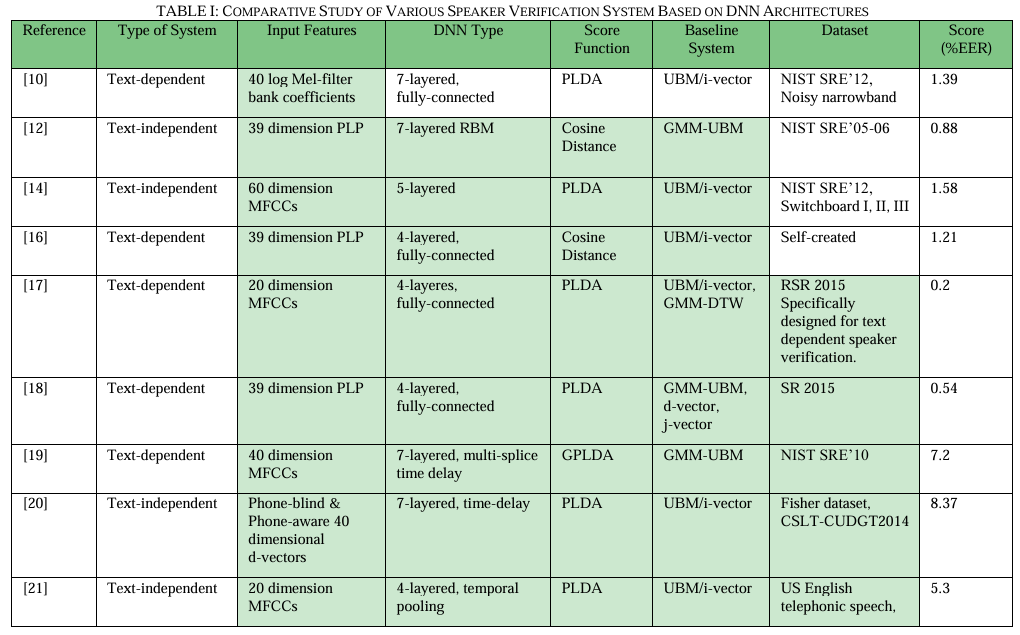
\includegraphics[width=1.0\textwidth]{./ch3/studio.png}
    \caption{Overview del Deep Learning applicato al problema, \cite{irum2019speaker}}
    \label{fig:studiopaper}
\end{figure}

\section{Metodologia del progetto}
Per la realizzazione del progetto abbiamo esplorato diverse strade basate sul deep learning, partendo comunque dal problema della speaker identification. 
Difatti, sulla base della speaker identification, possiamo poi usare la rete basata su deep learning stessa per poter identificare correttamente 
un utente tramite classificazione in termini di closed-set. Dopodiché siamo passati al task di speaker verification, partendo però dal modello addestrato che adesso funzionerà
da generatore di embeddings. Con questi embeddings costruiamo un modello GMM-UBM sulla base dei nostri utenti conosciuti, e valutiamo su utenti non conosciuti,
tramite scores di similarità valutando il rapporto di verosimiglianza. Per valutare il ratio di accettazione o rifiuto, il sistema calcola un valore di soglia che permette di definire il valore di EER
ottimale, ricordando che EER viene valutato quando FAR (False Acceptance Rate) e FRR (False Rejection Rate). \\

\section{Architettura Proposta}
Uno schema esemplificato della metodologia applicata è riportata in Fig.\ref{fig:architettura}.
Lo schema prevede una prima fase iniziale di Speaker Identification, dove a partire dagli speakers autorizzati (closed-set), estraiamo
features (ad esempio MFCCs) ed addestriamo uno speaker models basato su Deep Learning. Dopodiché, lo stesso modello verrà usato come estrattore di embeddings
per poter successivamente addestrare un modello di GMM-UBM (Universal Background Model, il nostro backend) per poter realizzare un sistema che permetta di fare
acceptance o rejection di speakers non autorizzati. L'idea generale è quello di applicare quanto fatto finora in letteratura per poter unire i due task in uno unico,
riconoscendo i nostri utenti e poi fare classificazione ed associazione.
\begin{figure}[ht]
    \centering
    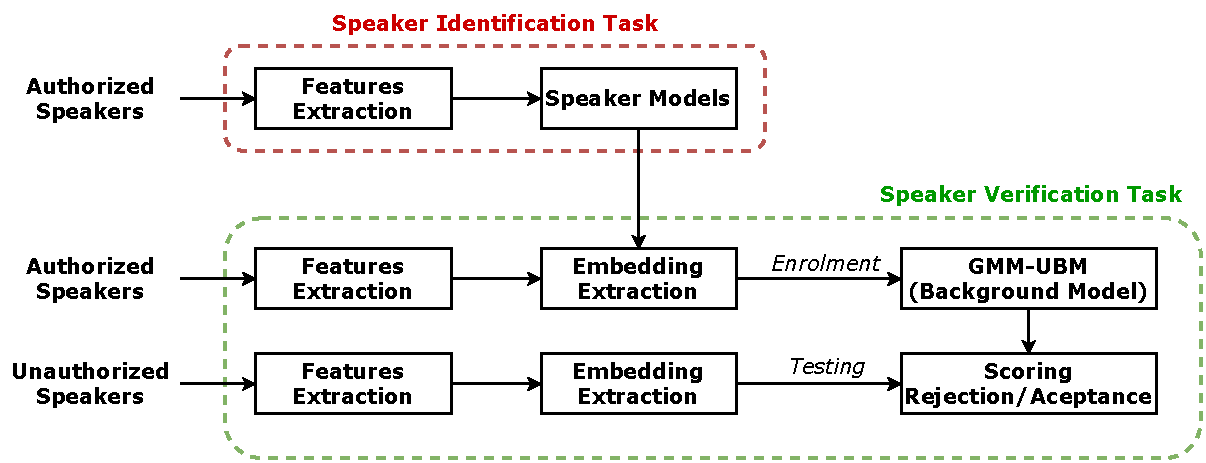
\includegraphics[width=1.0\textwidth]{./architettura.pdf}
    \caption{Architettura del progetto proposta}
    \label{fig:architettura}
\end{figure}
Per quanto riguarda lo score ci basiamo su un valore di soglia sull'EER (Equal Error Rate). La soglia viene utilizzata per decidere quando classificare un'istanza come genuina o impostore. Nel contesto di un sistema di autenticazione biometrica o di rilevamento delle frodi, la soglia è il valore sopra o sotto il quale una decisione viene presa.
Calcolo della soglia (Threshold) alla Equal Error Rate (EER), ovvero il punto in cui il tasso di falsi positivi (FPR) e il tasso di falsi negativi (FNR = 1 - TPR) sono uguali. Si identifica il valore della soglia corrispondente al punto in cui ( FPR - FNR ) è minimo.
Dopo aver calcolato la soglia all'EER, questa viene utilizzata per prendere decisioni di classificazione:
\begin{itemize}
    \item Se il punteggio di un campione è superiore alla soglia, viene considerato normale (positivo)
    \item Se è inferiore alla soglia, viene considerato impostore
\end{itemize}
Un particolare utilizzo di questo sistema potrebbe essere quello di un sistema di riconoscimento biometrico di una azienda, dove solo alcuni dipendenti
sono autorizzati ad accedere (controllo degli accessi), mentre gli altri non devono accedere. E qualora un utente dovesse essere autorizzato ad accedere,
quindi viene verificata la sua identità, il sistema di identificazione associerà un ID che permette di associare a quell'utente i privilegi specifici. \\
\newpage 
\chapter{Sezione Sperimentale}
\label{ch:esperimenti}

\section{Dataset utilizzato}
Per quanto riguarda i dataset, è stata condotta una prima fase di ricerca che portato all'utilizzo di LibriSpeech.
LibriSpeech è un dataset audio utilizzato per l’addestramento e la valutazione di modelli di automatic speech recognition (ASR). Il suo punto di forza è la grande quantità di dati disponibili, derivati da audiolibri di pubblico dominio, 
il che lo rende ideale per sviluppare sistemi che comprendano l’inglese parlato in modo naturale. Sono presenti speakers differenti,
bilanciati in termini di sesso e di durata delle tracce audio. Gli audio vengono forniti già normalizzati e puliti da eventuale rumore.
Il dataset è molto adatto per task di Speaker identification e verification in quanto gli audio sono molto chiari e ben distinguibili. \\
I file audio che compongono LibriSpeech provengono dagli audiolibri registrati nel progetto LibriVox, una piattaforma dove volontari 
leggono e registrano opere letterarie di dominio pubblico. Grazie a questa fonte, il dataset offre un ampio spettro di voci, con 
accenti e tonalità diverse, riflettendo meglio la variabilità del parlato umano, permettendo quindi di avere dati il quanto più
possibili generalizzanti.

\section{Dettagli Esperimenti}
In termini implementativi, per quanto riguarda i vari moduli o componenti, le configurazioni sono riportate in tabella Tab.\ref{tab:esperimenticondotti}.
\begin{table}[ht]
    \centering
    \resizebox{\textwidth}{!}{%
        \begin{tabular}{|ll|l|ll|}
        \hline
        \multicolumn{2}{|c|}{\textit{\textbf{Feature Extraction}}} & \multicolumn{1}{c|}{\textit{\textbf{Speaker Identification}}} & \multicolumn{2}{c|}{\textit{\textbf{Speaker Verification}}} \\ \hline
        \multicolumn{1}{|l|}{\textbf{Features used}} & \textbf{Frame Analysis} & \textbf{Model Used} & \multicolumn{1}{l|}{\textbf{Embedding}} & \textbf{Backend} \\ \hline
        \multicolumn{1}{|l|}{25 MFCCs} & \begin{tabular}[c]{@{}l@{}}25ms frame length\\ 10ms frame hop\end{tabular} & DNN & \multicolumn{1}{l|}{Bottle-neck layer} & GMM-UBM \\ \hline
        \multicolumn{1}{|l|}{25 MFCCs} & \begin{tabular}[c]{@{}l@{}}25ms frame length\\ 10ms frame hop\end{tabular} & DNN & \multicolumn{1}{l|}{Last Hidden layer} & GMM-UBM \\ \hline
        \multicolumn{1}{|l|}{25 MFCCs} & \begin{tabular}[c]{@{}l@{}}25ms frame length\\ 10ms frame hop\end{tabular} & RNN & \multicolumn{1}{l|}{Mean Hidden Layers} & GMM-UBM \\ \hline
        \multicolumn{1}{|l|}{25 MFCCs} & \begin{tabular}[c]{@{}l@{}}25ms frame length\\ 10ms frame hop\end{tabular} & CNN+LSTM & \multicolumn{1}{l|}{Mean Hidden Layers} & GMM-UBM \\ \hline
        \multicolumn{1}{|l|}{20 MFCCs} & \begin{tabular}[c]{@{}l@{}}25ms frame length\\ 10ms frame hop\end{tabular} & I-DNN & \multicolumn{1}{l|}{Segment Embedding} & GMM-UBM \\ \hline
        \multicolumn{1}{|l|}{\begin{tabular}[c]{@{}l@{}}24 MFCCs, \\ 24 Delta-MFCCs\\ VAD 30\% energy\end{tabular}} & \begin{tabular}[c]{@{}l@{}}25ms frame length\\ 10ms frame hop\end{tabular} & TDNN & \multicolumn{1}{l|}{X-embedding} & GMM-UBM \\ \hline
        \end{tabular}%
    }
\caption{Riassunto degli esperimenti condotti}
\label{tab:esperimenticondotti}
\end{table}
In particolare si è voluto dare maggior enfasi alla sperimentazione di diversi modelli,
diversi embedding e sopratutto features differenti. Ogni modello viene addestrato su un training e testing set comune, composto dagli audio
degli speaker autorizzati della top 10 di uomini e donne. Come si evince dalla tabella, per quanto riguarda le speech features da dare
in input ai modelli comunque applichiamo analisi short-time. L'analisi short-time deriva dal fatto che vogliamo
estrarre le caratteristiche di uno speaker a livello di frame (che possiamo pensare ad un singolo fonema), cercando di estrarre le features spaziali
e temporali caratteristiche. Proprio per questa possibilità, applichiamo diversi modelli che cercano ognuno di catturare questi aspetti. 
In particolare,per quanto riguarda la I-DNN, ispirata alla rete utilizzata per il calcolo degli I-Embeddings, validi sostituti degli I-Vectors (obsoleti e superati),
descritta in \cite{snyder2017deep}, andiamo ad estrarre embedding a livello di segmento, oltre che di singolo frames. Invece, gli X-Embedding si basano più
sulla rete descritta in \cite{snyder2018x}, ovvero una Temporal Delay Neural Network. 

\section{Risultati sperimentali}
Di seguito verranno riportate sia i risultati della Speaker Identification che Speaker Verification (in termini di EER).
Per quanto riguarda i risultati della prima, si riporta nel complessivo le prestazioni del sistema in termini di macro F1,Accuracy, e Precision
mentre i risultati sulla precisione del singolo speaker sono salvati nei rispettivi notebook python. Discorso analogo per quanto rigaurda il valore di EER.
\begin{table}[ht]
\resizebox{\textwidth}{!}{%
\begin{tabular}{|ll|l|lll|}
\hline
\multicolumn{2}{|c|}{\textit{\textbf{Feature Extraction}}} & \multicolumn{1}{c|}{\textit{\textbf{Speaker Identification}}} & \multicolumn{3}{l|}{\textit{\textbf{Metriche}}} \\ \hline
\multicolumn{1}{|l|}{\textbf{Features used}} & \textbf{Frame Analysis} & \textbf{Model Used} & \multicolumn{1}{l|}{\textbf{Acc}} & \multicolumn{1}{l|}{\textbf{F1}} & \textbf{Precision} \\ \hline
\multicolumn{1}{|l|}{25 MFCCs} & \begin{tabular}[c]{@{}l@{}}25ms frame length\\ 10ms frame hop\end{tabular} & DNN & \multicolumn{1}{l|}{1.0} & \multicolumn{1}{l|}{1.0} & 1.0 \\ \hline
\multicolumn{1}{|l|}{25 MFCCs} & \begin{tabular}[c]{@{}l@{}}25ms frame length\\ 10ms frame hop\end{tabular} & DNN & \multicolumn{1}{l|}{1.0} & \multicolumn{1}{l|}{1.0} & 1.0 \\ \hline
\multicolumn{1}{|l|}{25 MFCCs} & \begin{tabular}[c]{@{}l@{}}25ms frame length\\ 10ms frame hop\end{tabular} & RNN & \multicolumn{1}{l|}{0.97} & \multicolumn{1}{l|}{0.96} & 0.97 \\ \hline
\multicolumn{1}{|l|}{25 MFCCs} & \begin{tabular}[c]{@{}l@{}}25ms frame length\\ 10ms frame hop\end{tabular} & CNN+LSTM & \multicolumn{1}{l|}{0.99} & \multicolumn{1}{l|}{0.99} & 0.99 \\ \hline
\multicolumn{1}{|l|}{20 MFCCs} & \begin{tabular}[c]{@{}l@{}}25ms frame length\\ 10ms frame hop\end{tabular} & I-DNN & \multicolumn{1}{l|}{0.98} & \multicolumn{1}{l|}{0.98} & 0.98 \\ \hline
\multicolumn{1}{|l|}{\begin{tabular}[c]{@{}l@{}}24 MFCCs, \\ 24 Delta-MFCCs\\ VAD 30\% energy\end{tabular}} & \begin{tabular}[c]{@{}l@{}}25ms frame length\\ 10ms frame hop\end{tabular} & TDNN & \multicolumn{1}{l|}{0.94} & \multicolumn{1}{l|}{0.94} & 0.95 \\ \hline
\end{tabular}%
}
\caption{Speaker Identification}
\label{tab:speakeridresult}
\end{table}

\begin{table}[ht]
\resizebox{\textwidth}{!}{%
\begin{tabular}{|ll|l|ll|l|}
\hline
\multicolumn{2}{|c|}{\textit{\textbf{Feature Extraction}}} & \multicolumn{1}{c|}{\textit{\textbf{Speaker Identification}}} & \multicolumn{2}{l|}{\textit{\textbf{Speaker Verification}}} & \multicolumn{1}{c|}{\textit{\textbf{Metrics}}} \\ \hline
\multicolumn{1}{|l|}{\textbf{Features used}} & \textbf{Frame Analysis} & \textbf{Model Used} & \multicolumn{1}{l|}{\textbf{Embedding}} & \textbf{Backend} & \textbf{EER} \\ \hline
\multicolumn{1}{|l|}{25 MFCCs} & \begin{tabular}[c]{@{}l@{}}25ms frame length\\ 10ms frame hop\end{tabular} & DNN & \multicolumn{1}{l|}{Bottle-neck layer} & GMM-UBM & 0.03 \\ \hline
\multicolumn{1}{|l|}{25 MFCCs} & \begin{tabular}[c]{@{}l@{}}25ms frame length\\ 10ms frame hop\end{tabular} & DNN & \multicolumn{1}{l|}{Last Hidden layer} & GMM-UBM & 0.13 \\ \hline
\multicolumn{1}{|l|}{25 MFCCs} & \begin{tabular}[c]{@{}l@{}}25ms frame length\\ 10ms frame hop\end{tabular} & RNN & \multicolumn{1}{l|}{Mean Hidden Layers} & GMM-UBM & 0.12 \\ \hline
\multicolumn{1}{|l|}{25 MFCCs} & \begin{tabular}[c]{@{}l@{}}25ms frame length\\ 10ms frame hop\end{tabular} & CNN+LSTM & \multicolumn{1}{l|}{Mean Hidden Layers} & GMM-UBM & 0.15 \\ \hline
\multicolumn{1}{|l|}{20 MFCCs} & \begin{tabular}[c]{@{}l@{}}25ms frame length\\ 10ms frame hop\end{tabular} & I-DNN & \multicolumn{1}{l|}{I-embedding} & GMM-UBM & 0.16 \\ \hline
\multicolumn{1}{|l|}{\begin{tabular}[c]{@{}l@{}}24 MFCCs, \\ 24 Delta-MFCCs\\ VAD 30\% energy\end{tabular}} & \begin{tabular}[c]{@{}l@{}}25ms frame length\\ 10ms frame hop\end{tabular} & TDNN & \multicolumn{1}{l|}{X-embedding} & GMM-UBM & 0.48 \\ \hline
\end{tabular}%
}
\caption{Speaker Verification}
\label{tab:speakerverresults}
\end{table}

\begin{figure}[ht]
    \centering
    \begin{minipage}{0.47\textwidth}
        \centering
        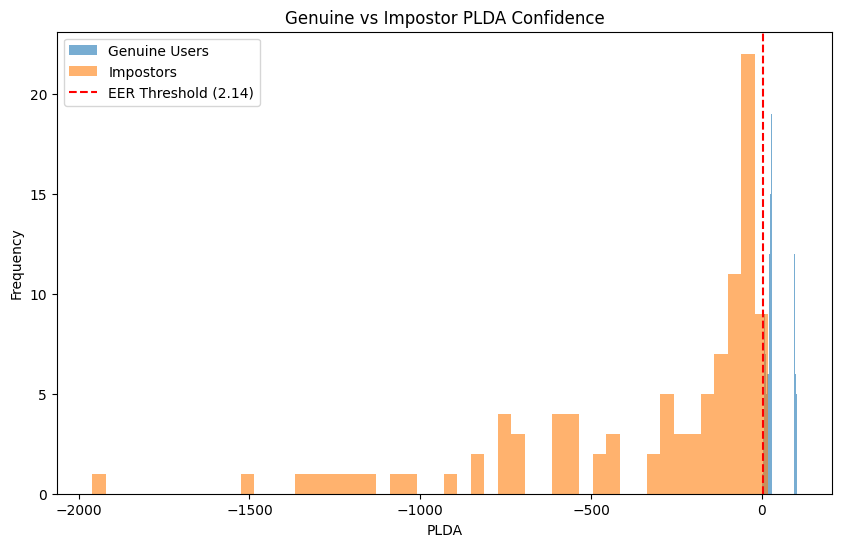
\includegraphics[width=\textwidth]{./ch4/dnn1.png}
        \caption{DNN (1)}
    \end{minipage}
    \begin{minipage}{0.47\textwidth}
        \centering
        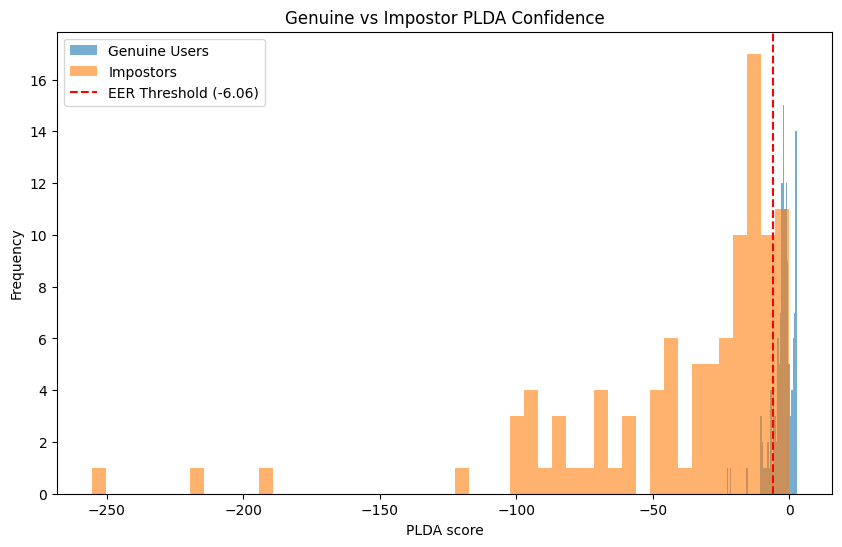
\includegraphics[width=\textwidth]{./ch4/dnn2.png}
        \caption{DNN (2)}
    \end{minipage}

    \begin{minipage}{0.47\textwidth}
        \centering
        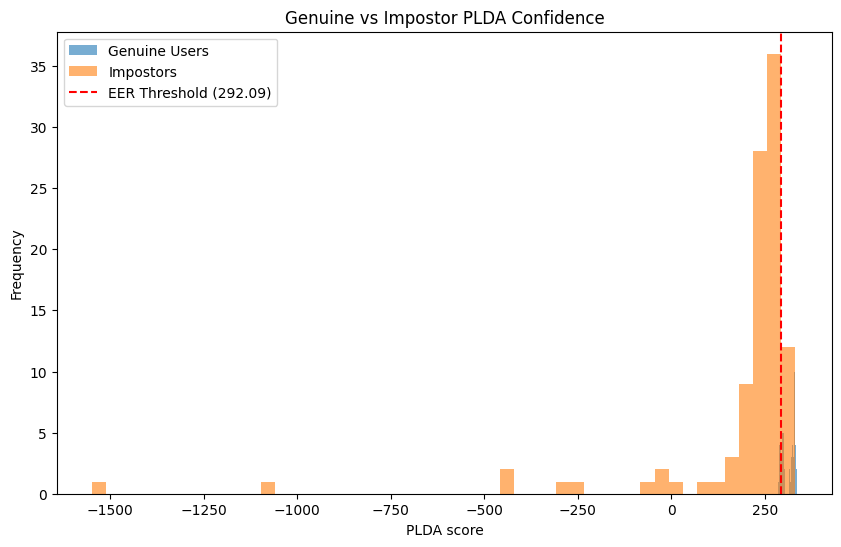
\includegraphics[width=\textwidth]{./ch4/rnn}
        \caption{RNN}
    \end{minipage}
    \begin{minipage}{0.47\textwidth}
        \centering
        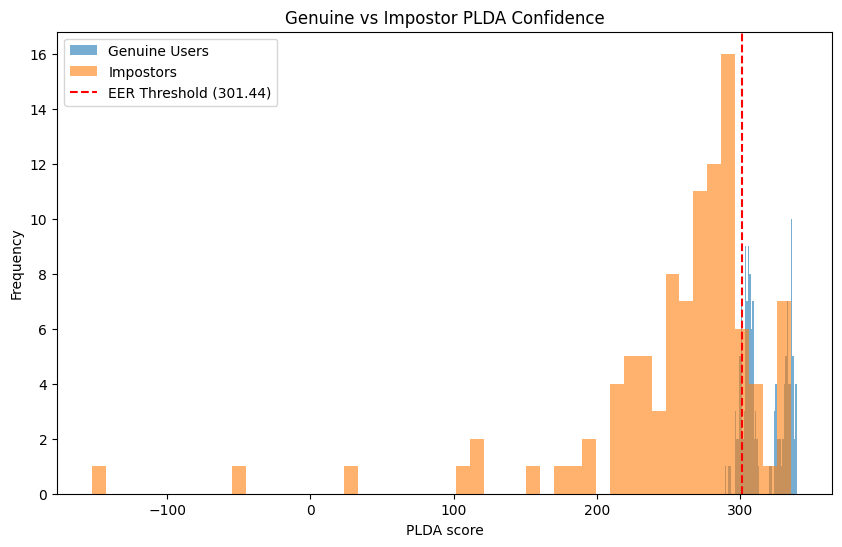
\includegraphics[width=\textwidth]{./ch4/cnnlstm.png}
        \caption{CNN+LSTM}
    \end{minipage}

    \begin{minipage}{0.47\textwidth}
        \centering
        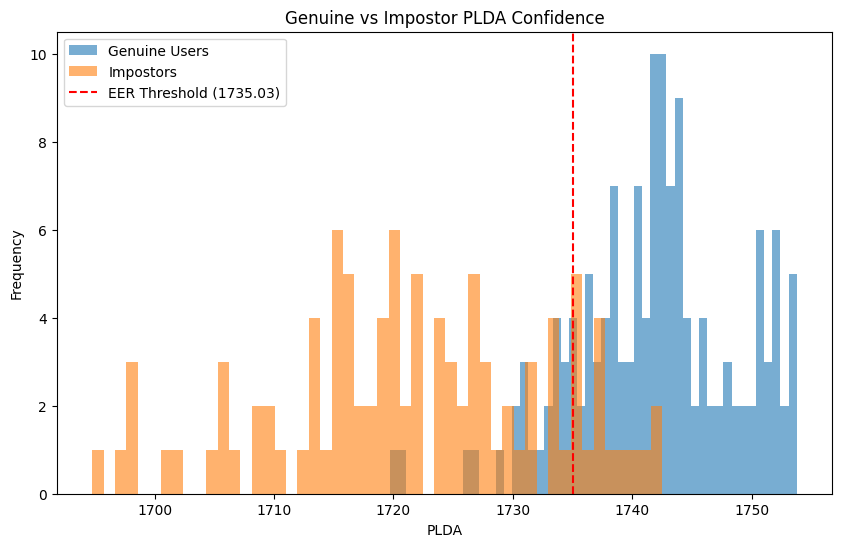
\includegraphics[width=\textwidth]{./ch4/idnn.png}
        \caption{I-DNN}
    \end{minipage}
    \begin{minipage}{0.47\textwidth}
        \centering
        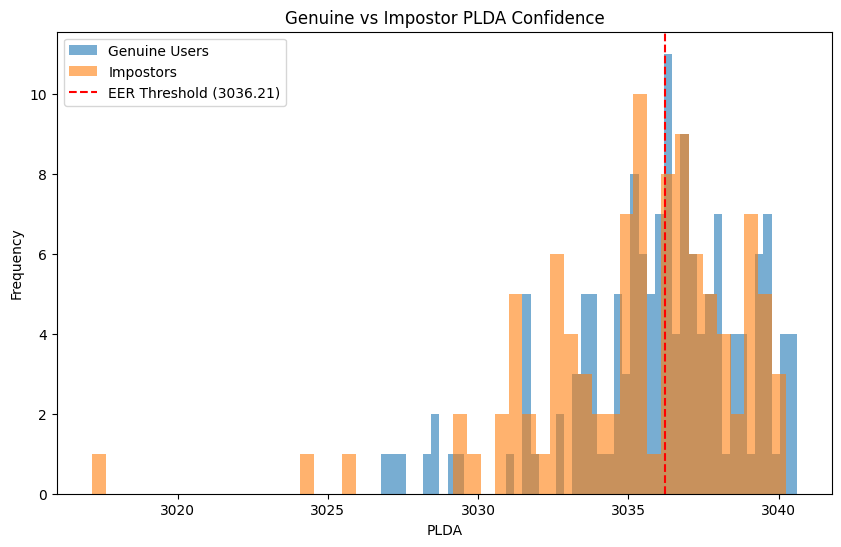
\includegraphics[width=\textwidth]{./ch4/xdnn.png}
        \caption{X-DNN}
    \end{minipage}
\end{figure}


\clearpage

\section{Conclusioni}
Alla luce delle sperimenazioni effettuate, dalla tabella Tab.\ref{tab:speakeridresult} vediamo come effettivamente
tutti i modelli si comportano molto bene nella identificazione degli utenti. Tuttavia va precisato che la natura del dataset non è
di grandi dimensioni, difatti abbiamo a disposizione circa 100 audio per ogni speaker, il che sicuramente è molto limitante come numero. 
Tuttavia, è nella fase di sperimentazione della Speaker Verification (riportate in tabella Tab.\ref{tab:speakerverresults}) dove notiamo che la 
legge del rasoio di Occam non delude mai: difatti la rete che presenta le migliori prestazioni sembra essere la DNN tradizionale cone 
estrazione degli embedding dal Bottleneck.

Difatti entrambe le DNN presentate anche in termini di distribuzione degli scores da parte del backend (vedi Fig.5.1 e Fig.5.2) sia molto precisa
nel trovare embedding abbastanza discriminanti. Discorso diverso invece va fatto per le due ultime reti,
I-DNN e X-DNN, dove vediamo che la distribuzione è abbastanza spalmata e sovrapposta, sintomo che la rete non riesce ancora bene a distinguere. Questo 
lo possiamo notare sopratutto dove la X-DNN riporta il peggior risultato in termini di EER. Questo potrebbe essere dovuto al fatto che la rete
presenta un numero di parametri abbastanza elevato e rischia di overfittare quasi subito, andando difatti a riconoscere bene gli speaker, ma nonr riuscendo
a discriminare quelli "reali" da quelli "estranei". 

Concluendo, possiamo dire che questi sistemi basati su deep learning sul dataset attualmente in uso permettono in maniera precisa di identificare gli speaker,
quindi si prestano molto bene per task in closed-set, ma non possiamo sicuramente dire lo stesso per quanto riguarda il sistema di verifica, che presenta un EER troppo alto,
sintomo che ci sarebbero tanti falsi positivi che riuscirebbero ad entrare nel sistema, venendo identificati erroneamente come utenti legittimi

\printbibliography

\end{document}
